\chapter{Implementation}
\label{chap:Impl}
\section{Programming APIs}

To implement VR applications, we can work directly with the SDK provided by each headset manufacturer. The advantage is that we can interact at a low level with the devices. 
Another way is to use an SDK of a well-defined standard for example OpenVR from Valve \cite{OpenVRValve} or OpenXR from the Khronos Group \cite{khronosGroupOpenXR}. This allows us to write applications for a target group of devices like 6-DOF supporting headsets without having to deal with different manufacturer SDKs (see Figure \ref{fig:openxr-overview}). On a side note: the X in OpenXR means that the specification is not only used for virtual reality (VR) applications but also for augmented reality (AR) and other technologies (XR) possibly proposed in the future.
Lastly, we can work with different 3D graphic engines which provide various additional features. While classical desktop engines rely on downloading a complete bundled software package for distributing the application, browser based engines like A-Frame \cite{aframe} that use WebXR \cite{webxr} and WebVR \cite{webvr} allow us to distribute and run our application via the browser, similarly to WebGL.

At the time of writing, the OpenXR and WebXR specification is still relatively new being in its first revision. Therefore, it is not implemented by each headset manufacturer, browser and engine yet. However, these standards are meant to replace the old OpenVR and WebVR in the future.

\begin{figure}[!hbt]
    \centering
    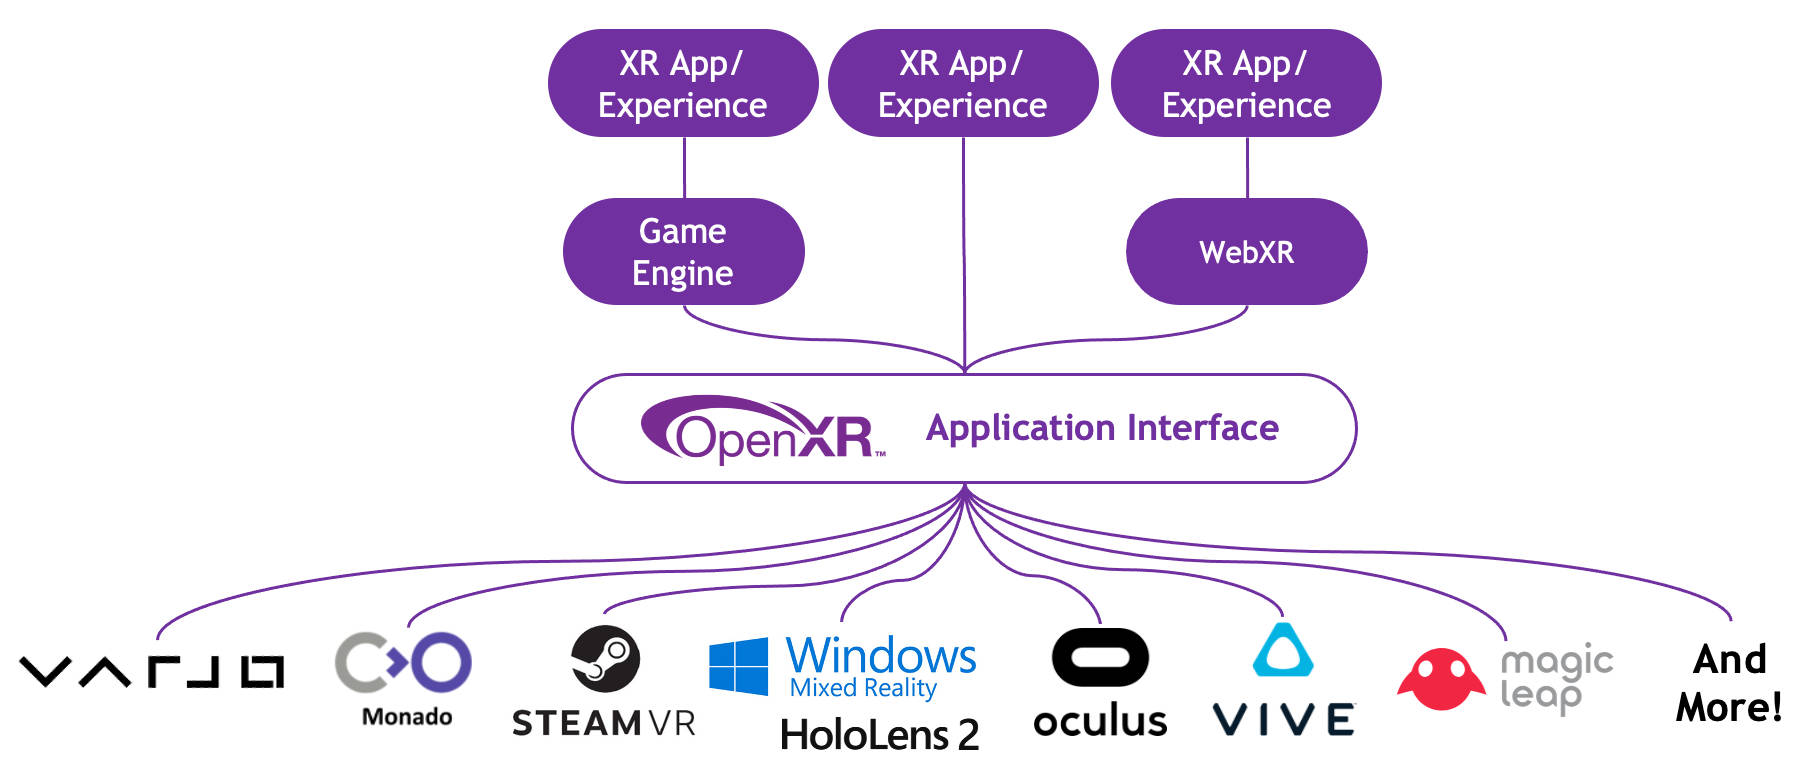
\includegraphics[width=\textwidth]{graphics/openXR-overview.jpg}
    \caption{Overview of the OpenXR API Stack \cite{khronosGroupOpenXR}.}
    \label{fig:openxr-overview}
\end{figure}

\section{Prior Publication}
For our implementation, we extend the code of a prior publication from Sorger et al. \cite{sorger_immersive_2019}. 
They implemented an immersive visualization for node-link networks that does not explicitly support hierarchical network data. Their implementation already contains a common force-based layout, the laser-pointer ray casting technique to select objects, free flying as well as animated teleport navigation and lastly a code structure with an included render engine. A screenshot of their work is shown in Figure \ref{fig:priorPublication}.\\
We extended their implementation by adding the ability to visualize and interact with hierarchical networks as described in Section \ref{chap:proposed-Solution}. To achieve that, we had to adapt the layout algorithm, add transparent rendering, change the target position for the animated teleport, change the controller button mappings, implement the link filtering technique, add automatic/manual scaling of the virtual scene and automatic/manual adaption of the free flying speed.
This process is described in detail in Section \ref{sec:applOverview} and \ref{sec:applDetails}.

\begin{figure}[!hbt]
    \centering
    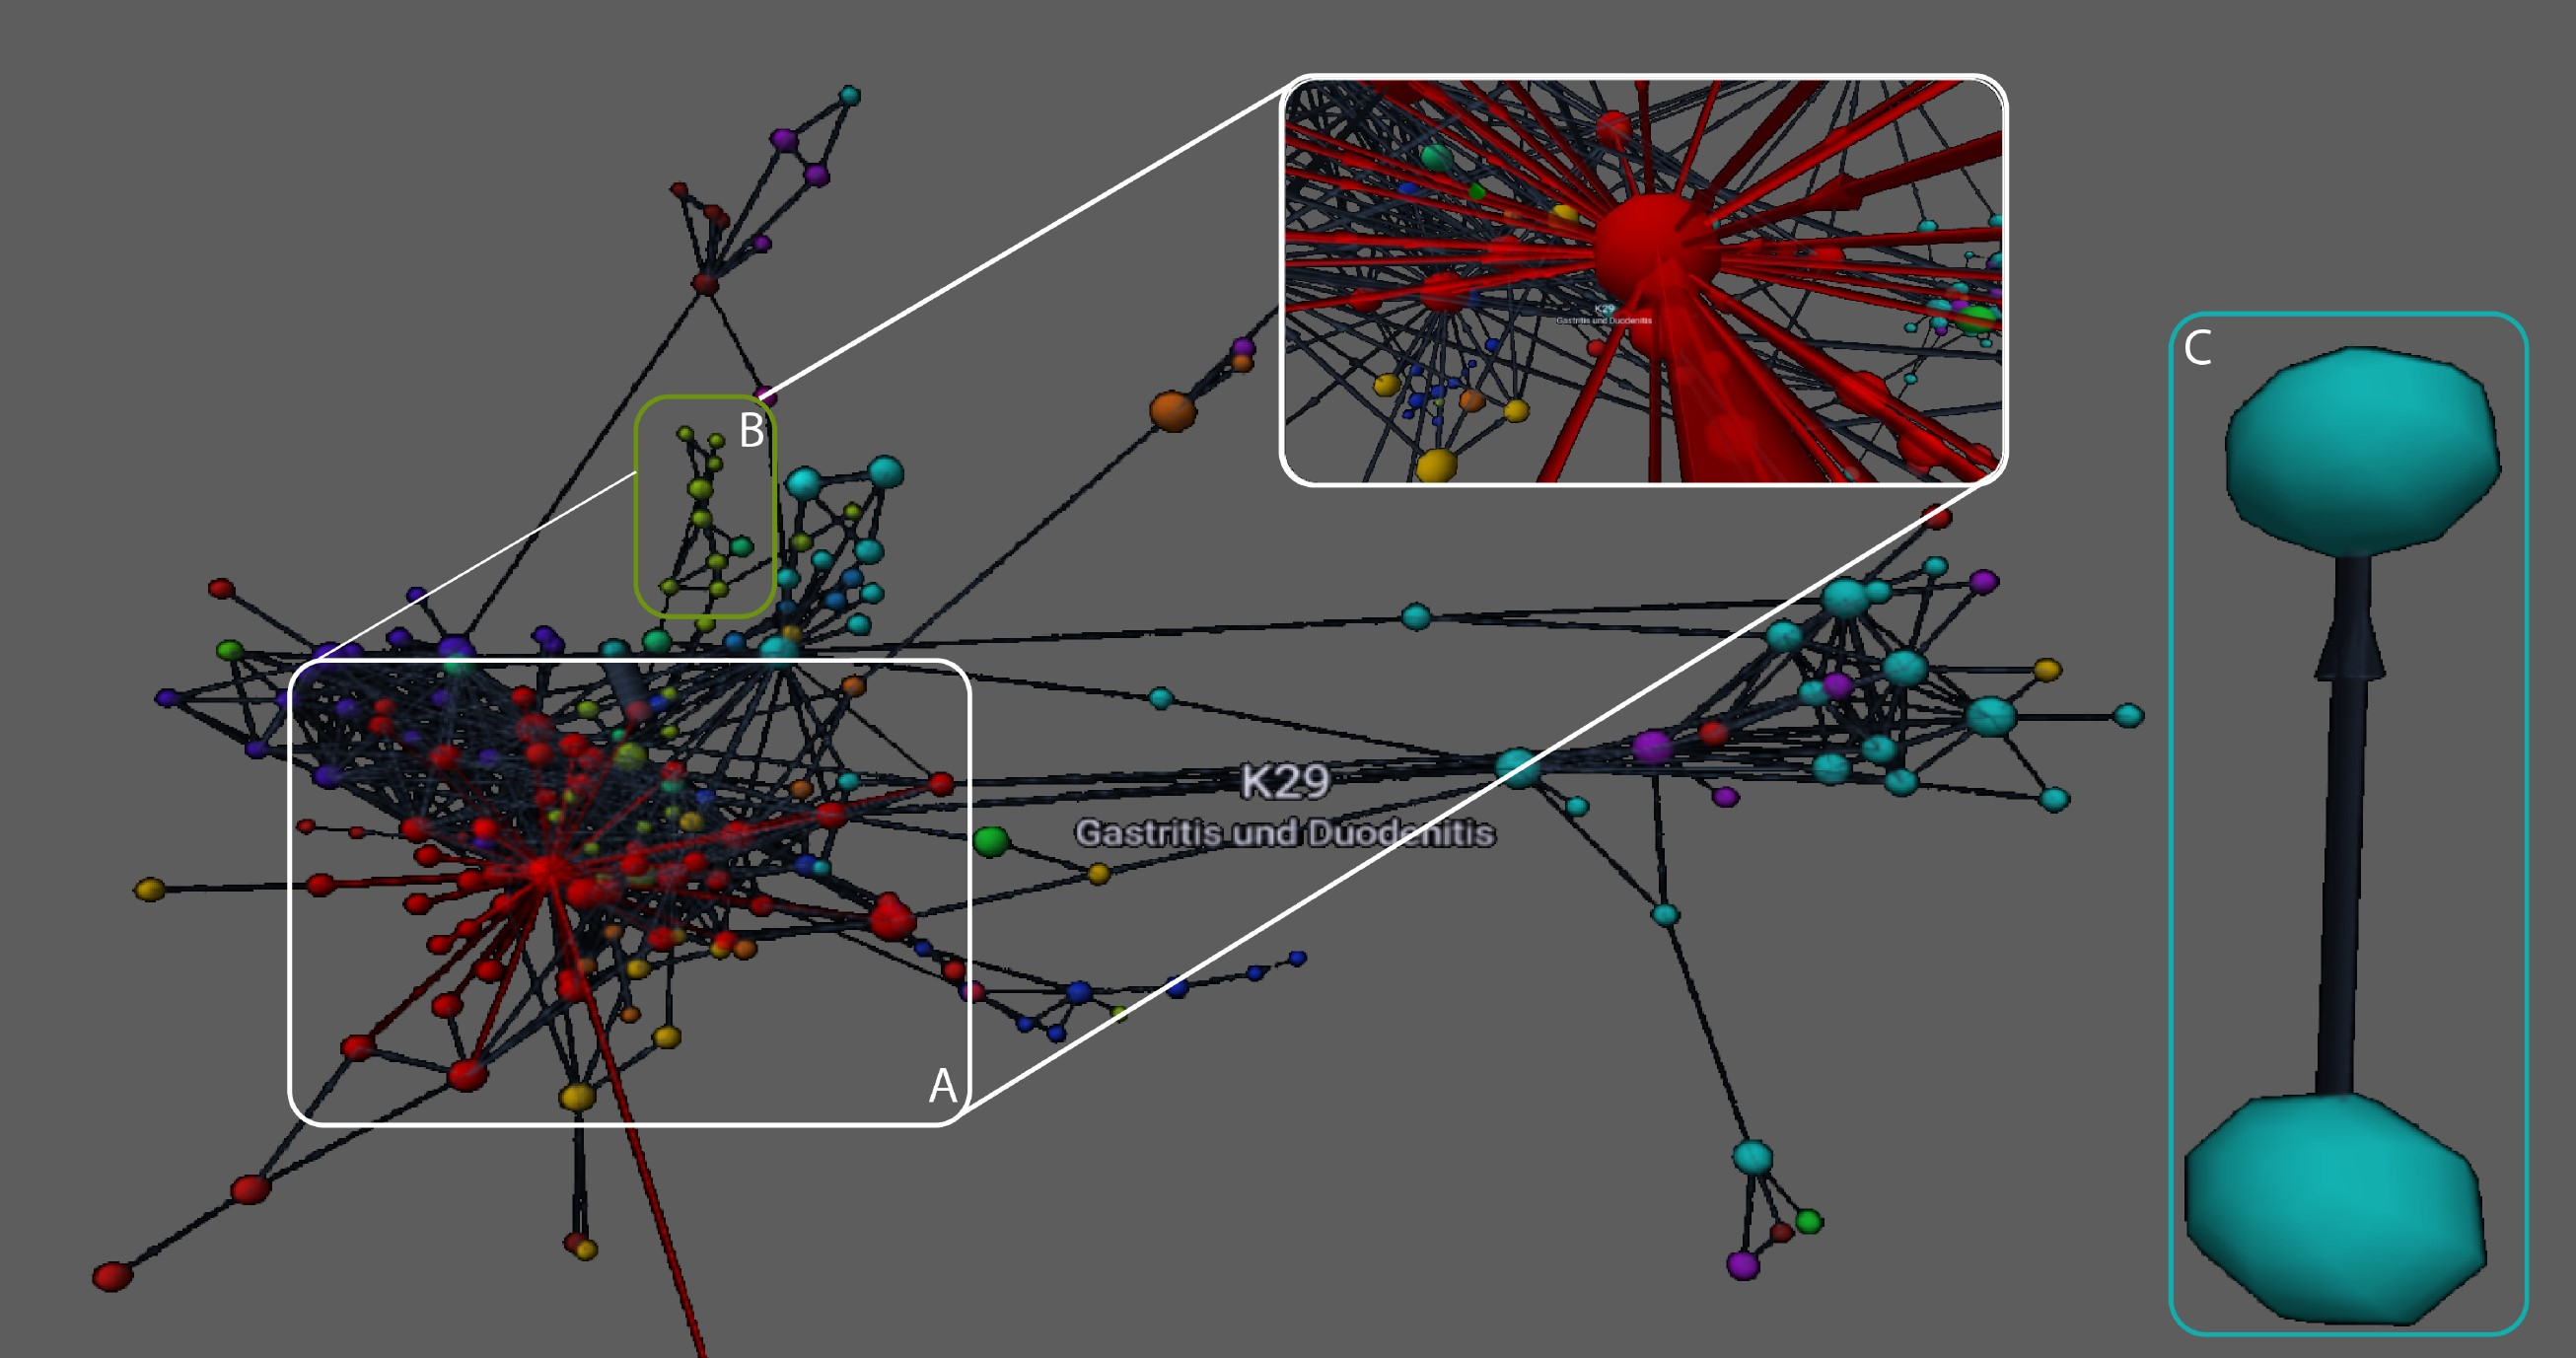
\includegraphics[width=\textwidth]{graphics/screenshotPriorPublication.jpg}
    \caption{Screenshot of the visualization from Sorger et al. \cite{sorger_immersive_2019} we extend our implementation on.}
    \label{fig:priorPublication}
\end{figure}

\section{Technology}

The application is implemented in plain JavaScript and runs in browsers that support the WebVR standard. 
At the time of writing, this only applies to Firefox for Windows (our tested version is 85.0.2 (64-Bit)). 
In order to reduce the complexity for rendering and implementing the WebVR standard, the application uses the framework A-Frame \cite{aframe}. The code of the publication we extended uses A-Frame in version 0.9.2 from September 2019, which internally uses three.js \cite{threejs} in version 0.108.0 as a render engine.
This old version of A-Frame brings the limitation of only supporting WebVR because WebXR was not yet ready back in 2019.
Unfortunately, WebVR is already deprecated and being replaced with the new WebXR standard.
While we know that it is unlikely that other browser vendors will support WebVR in the future, we decided to not update the A-Frame version. Updating to a current version would break many features already implemented and a complete migration would not be possible within reasonable time. Therefore, we decided to stick to the old version and only support WebVR browsers and headsets.
The primary VR headset we are targeting with our application is the original HTC Vive.

\section{Application Overview}

\label{sec:applOverview}
\subsection{Data Structure}
\label{subSec:dataStruct}
To get a better understanding of the implementation, we begin with describing the data structure for storing the graph.
Listing \ref{lst:internalJSON} shows a minimalistic example of the data structure that we use an input data source. The data is formatted as a JSON object with a flat list of nodes and links. The hierarchical information is encoded within the attributes childNodesIDs and parentNodeID as references. 
In addition to the necessary attributes, each node and link object can have additional attributes depending on the specific dataset.

\pagebreak

\begin{lstlisting}[language=json,label={lst:internalJSON},caption={minimal JSON input data structure. The id attribute has to follow the pattern ”<layerNr>.<uniqueNodeIDByLayer>”. The desc, color and weight attribute can be set individually. Besides these required properties there can be any number of additional properties.}]
{
    "nodes": [
        {
            "id": "0.0",
            "weight": 4.5,
            "color": "rgb(77, 175, 74)",
            "layer": "0",
            "desc": "0.0",
            "childNodeIDs": [
                "1.1",
                "1.3",
                ...
            ]
        },
        ...
        {
            "id": "1.1",
            "weight": 1.7,
            "color": "rgb(250, 250, 110)",
            "layer": "1",
            "desc": "1.1",
            "parentNodeID": "0.0",
            "childNodeIDs": [
                "2.1",
                ...
            ]
        },
        ...
    ],
    "links": [
        {
            "color": "rgb(77, 175, 74)",
            "layer": "0",
            "source": "0.0",
            "target": "0.1",
            "label": "0.0 - 0.1",
            "linkwidth": 0.35
        },
        ...
    ]
}
\end{lstlisting}

\subsection{Program Flow}
\label{section:programFlow}
\begin{figure}[!hbt]
    \centering
    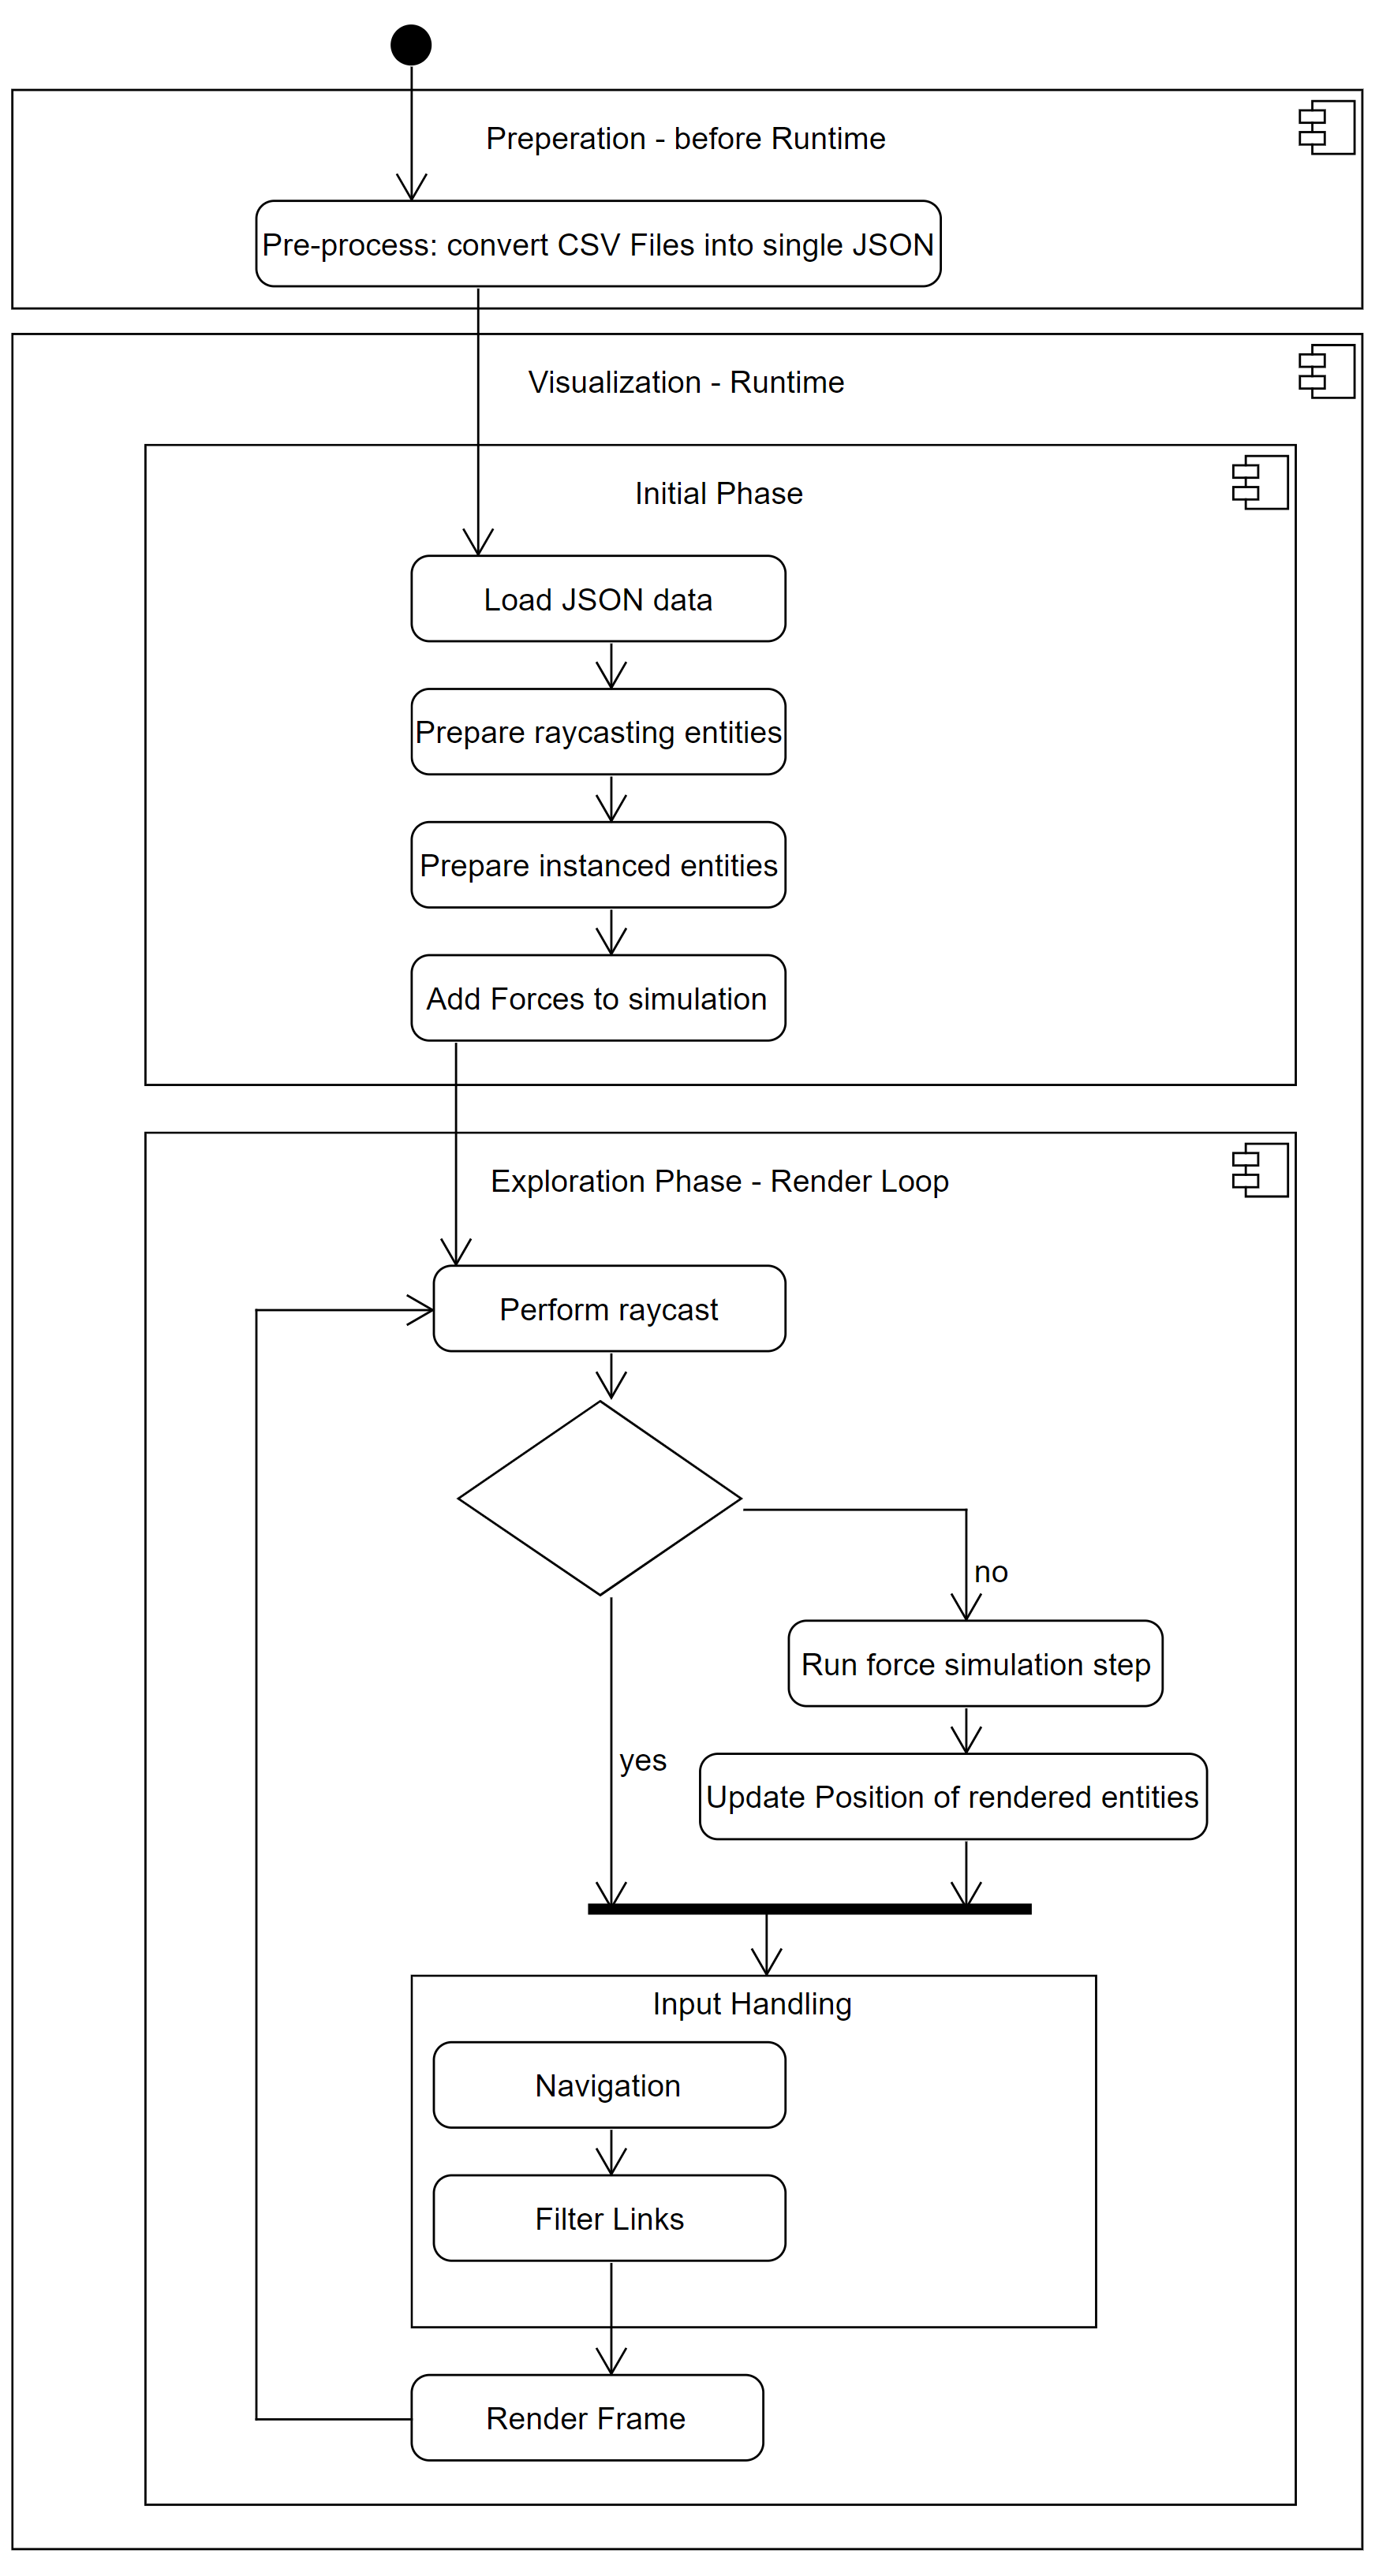
\includegraphics[width=0.70\textwidth]{graphics/vrgraph_flow.png}
    \caption{Sequence diagram of the program flow for our application.}
    \label{fig:impl_programFlow}
\end{figure}

We separated the application into multiple processing steps. Figure \ref{fig:impl_programFlow} describes the program flow and all abstract steps that are necessary for the visualization.
It consists of an offline preparation phase where the graph data is converted once to our internal JSON data structure (see Section \ref{sec:preprocessing}) and a runtime phase, which is executed every time the browser loads the webpage.
The runtime phase starts with loading the data, afterwards preparations for the instanced rendering (see Section \ref{sec:rendering}) and the force based layout (see Section \ref{sec:layoutCalculation}) are carried out.
Then, the main render loop is executed, which produces a rendered frame for each interaction. In addition, the layout calculation (see Section \ref{sec:layoutCalculation}), navigation methods (see Section \ref{sec:vrInteractions}), scaling (see Section \ref{sec:scaling}), filtering visible links (see Section \ref{sec:linkFiltering}) and performing the ray casting for the virtual laser pointer is handled by the main render loop.
The objects that are intersected by the virtual laser pointer are used in the navigation and interaction techniques. 
Details on how intersected objects are determined by ray casting is not further described as this method is already provided from the original implementation. 

\subsection{Virtual Scene Graph}
A-Frame applications are built by creating a virtual scene graph.
The framework uses an entity-component-system architecture, which follows the “composition over inheritance and hierarchy” principle. 
This means that every object in A-Frame is an entity that can be extended and customized.
There are various components that can be reused and extended. The base component is represented by the <a-entity> element.\\
Listing \ref{lst:virtualSceneGraph} shows a simplified version of the virtual scene graph the application uses. 
It consists of entities for both Vive controllers, a passive and active camera, the rig setup and the graph object itself.
Most data and logic is encapsulated in the graphData object. We maintain two types of data lists: a list of nodes/links for the ray casting entities and a list of nodes/links for the actual rendered entities. 
The reason for this duplicated data is that we use  instanced objects for rendering (see Section \ref{sec:rendering}) and these can not be used for ray casting directly.
\pagebreak

\begin{lstlisting}[label={lst:virtualSceneGraph},caption=Simplified virtual A-Frame scene graph used by the application.]
<body>
    <a-scene ... >
        <a-entity vive-controls="hand: left"> </a-entity>
        <a-entity vive-controls="hand: right"> </a-entity>
        
        <a-entity id="graphData" json-url="data/inputData.json" ... >
            <a-entity id="passive_rig"  ... >  
                <a-entity id="passive_cam" ... > </a-entity>
            </a-entity>
            ...
        </a-entity>

        <a-entity id="active_rig" ... >
            <a-text id="controllerLabel" ... > </a-text>
            <a-entity id="active_cam" ... > </a-entity>
        </a-entity>
        ...
    </a-scene>
</body>
\end{lstlisting}

\section{Application Details}
\label{sec:applDetails}
\subsection{Preprocessing Scripts}
\label{sec:preprocessing}

The visualization expects a combined JSON file with all nodes and links and their assigned layer as seen in Section \ref{subSec:dataStruct}.
A common data export format for networks are multiple CSV files: one file for the nodes and another for their edges.
In a hierarchical or clustered network, there can be an additional file with the hierarchical mapping.
Therefore, we needed a script to convert these CSV files to our JSON data format. For convenience, most parameters can be configured by an additional config file without changing any program code. 
While transforming the data structure, all node IDs are extended with their hierarchical layer information to ensure unique IDs for the entire dataset. The node with an ID 1 on hierarchical layer 0 is assigned the new ID 0.1.  
In addition, we also normalize the node and link width and add color attributes for a simplified rendering process.
To test our visualization with various networks of different sizes, there is also a script for generating test data.

\subsection{Automated Force Layout}
\label{sec:layoutCalculation}

The node layout is automatically calculated during runtime by a force system powered by D3-Force \cite{bostock_d3forcejs_nodate}. At the beginning, all D3-Force specific parameters including alphaDecay, alphaTarget, alphaMin, velocityDecay and cooldownTime are set. 
These parameters adjust the flexibility of the simulation by changing the strength behavior for all forces, how much the velocity is decreased between every simulation step and how many simulation steps are applied in total.
In a second step, we add all forces to the simulation. This process is shown in Listing \ref{lst:addForces}.
The center, many-body, link and collision forces use a slightly adapted version of the original implementation in D3 force. 
The spherical constraint is our own implementation which can be seen in Listing \ref{lst:sphericalConstraint}. The main goal here is to add a velocity for each child node depending on the current node position. This velocity pulls the nodes to the center of their parent node which allows us to achieve the proclaimed hierarchical nested layout.
Lastly, a simulation step is called every frame, which handles the subroutine calls for the different forces. The simulation is then stopped when a fixed number of steps is executed. The amount of simulation steps is determined by the alpha parameters set in the first step.

\begin{lstlisting}[language=JavaScript,label={lst:addForces},caption=Simplified algorithm that shows which forces are added to the simulation.] 
//add forces for hierarchical layer 0
d3ForceLayout.force("layer0-center",centerForce(...));
d3ForceLayout.force("layer0-link",linkForce(...))
d3ForceLayout.force("layer0-manyBody",manyBodyForce(...));
d3ForceLayout.force("layer0-collide",collideForce(...)));

//add forces for each parent node (layer 1-n)
parentNodeIDs.forEach((parentNodeID, index) => {
    const filteredNodesForLayer = filterNodes(nodes, function (d) {
        return d[parentNodeIDKey] === parentNodeID && parseInt(d.layer) === childLayer;
    })

    d3ForceLayout.force(parentNodeID + "-sphericalConstraint",sphericalConstraint(filteredNodesForLayer,...));
    d3ForceLayout.force(parentNodeID + "-forceCollision",collisionForce(filteredNodesForLayer,...));
    d3ForceLayout.force(parentNodeID+ "-manyBody",manyBodyForce(filteredNodesForLayer,...));
    d3ForceLayout.force(parentNodeID+ "-link",linkForce(filteredNodesForLayer,...));
});
\end{lstlisting}
\pagebreak


\begin{lstlisting}[language=JavaScript,label={lst:sphericalConstraint},caption=Simplified algorithm for the spherical constraint. We apply adapted velocities whenever the child node is inside the parent. We further determine if the childnode is already closer to the center of the node or not.] 
nodes.forEach(node => {
    let layerInt = parseInt(node.layer);

    let diffX = node.x - parentNode.x;//distance to the center
    let velocityDiffX;
    if(Math.abs(diffX) < radius){//child is inside parent
        if (Math.abs(diffX) < innerRadius) {//node is already close to the center
            velocityDiffX = diffX * jiggle(layerInt * const);
            //jiggle provides a randomized value
        }else{
            velocityDiffX = diffX * strength / const;
        } 
    }else{//child is outside parent
        velocityDiffX = diffX * strength + jiggle(layerInt);
    }
    //Add velocity towards the center of the parent node
    node.vx -= (velocityDiffX/constant);
    //Add alpha value to allow the simulation to 'cool down'
    node.vx *= (1-alpha);
    ... (same for y,z)
}
\end{lstlisting}

\subsection{Rendering}
\label{sec:rendering}

There are multiple goals for the rendering part, one of them is to increase the performance for large graphs. 
To achieve such FPS improvement, the application uses instanced rendering for nodes and links. This means that there is not one 3D object for every node/link in the virtual scene. Instead, we group multiple items and render them as a group. The final rendered position is then determined in the vertex shader, which reduces the overhead of draw calls from WebGL.
The implementation of the prior paper \cite{sorger_immersive_2019} used two instanced buffers: one for the nodes and one for the links. 
Another goal for the rendering was to use transparent nodes. This requires to create multiple instanced buffers for the nodes, one for each hierarchical layer. 
Therefore, enabling us to set the render order of the instanced buffers in ascending order according to the hierarchical layers. A correct render order ensures  a valid transparency so that child nodes can be seen from outside.

\subsection{VR Navigation}
\label{sec:vrInteractions}

As described in Section \ref{chap:solution-navigation} for navigation we provide two methods: free flying and an animated teleport.
Before we go into the details of the techniques, it is important to understand the core concept of navigation for 6-DOF VR headsets.
The camera is placed in a virtual camera rig, which represents the user's available movement space.
Programming guidelines from VR APIs prohibit programmatically changing the position of the headset or controllers in the rig as this would create confusion for the user. 
The only way the headset and controllers are moved inside the rig is by physical movement in the real world, thus enabling enable free walking inside the virtual rig.
Instead of the camera directly, we can programmatically change the position of the rig inside the virtual scene. 
We apply this technique for our free flying and teleport technique.
The free flying technique is already provided by A-Frame and the implementation from the prior paper.
We just added additional controller button callbacks for adapting the fly speed and rotate of the rig in the virtual scene on demand.
For the animated teleport technique, we no longer fly to the center of the selected node, as in the original implementation. Instead, the target position is the node border barely on the inside of the node. Therefore, we changed the calculation for the target position, which can be seen in Listing \ref{lst:calculationFlyToNode}. The process is also visualized in Figure \ref{fig:vrFlyToNode}.

\begin{lstlisting}[language=JavaScript,label={lst:calculationFlyToNode},caption=Matrix calculations for determining the target position of the animated teleport.]
//1. get all needed information
const nodePos = node.pos;
const nodeRadius = multilayerNodeDiameter(node.__data);
const sceneScale = detailLayout.getCurrentSceneScale() ;
let cameraPos = getCurrentCameraRigWorldPos().add(getRelativeCameraToRigPos());
//2. calculate the node border position between the camera and nodeCenter
const vecNodeToCamera = cameraPos.add(nodePos.clone().negate());
const vecCenterToNodeBorder = vecNodeToCamera.normalize().multiplyScalar(nodeRadius*0.95*sceneScale);//*0.95 as we want to be slightly inside the selected node
//3. convert position so that the headset instead of the rig is centered
const positionNodeBorder = nodePos.clone().add(vecCenterToNodeBorder);
const positionNodeBorderCorrectedWithCurrentCameraPos = positionNodeBorder.clone().add(getRelativeCameraToRigPos().negate());
//4. initiate animated teleport
flyToPosition(positionNodeBorderCorrectedWithCurrentCameraPos, flyingElement);
\end{lstlisting}
\pagebreak

\begin{figure}[h]
    \centering
    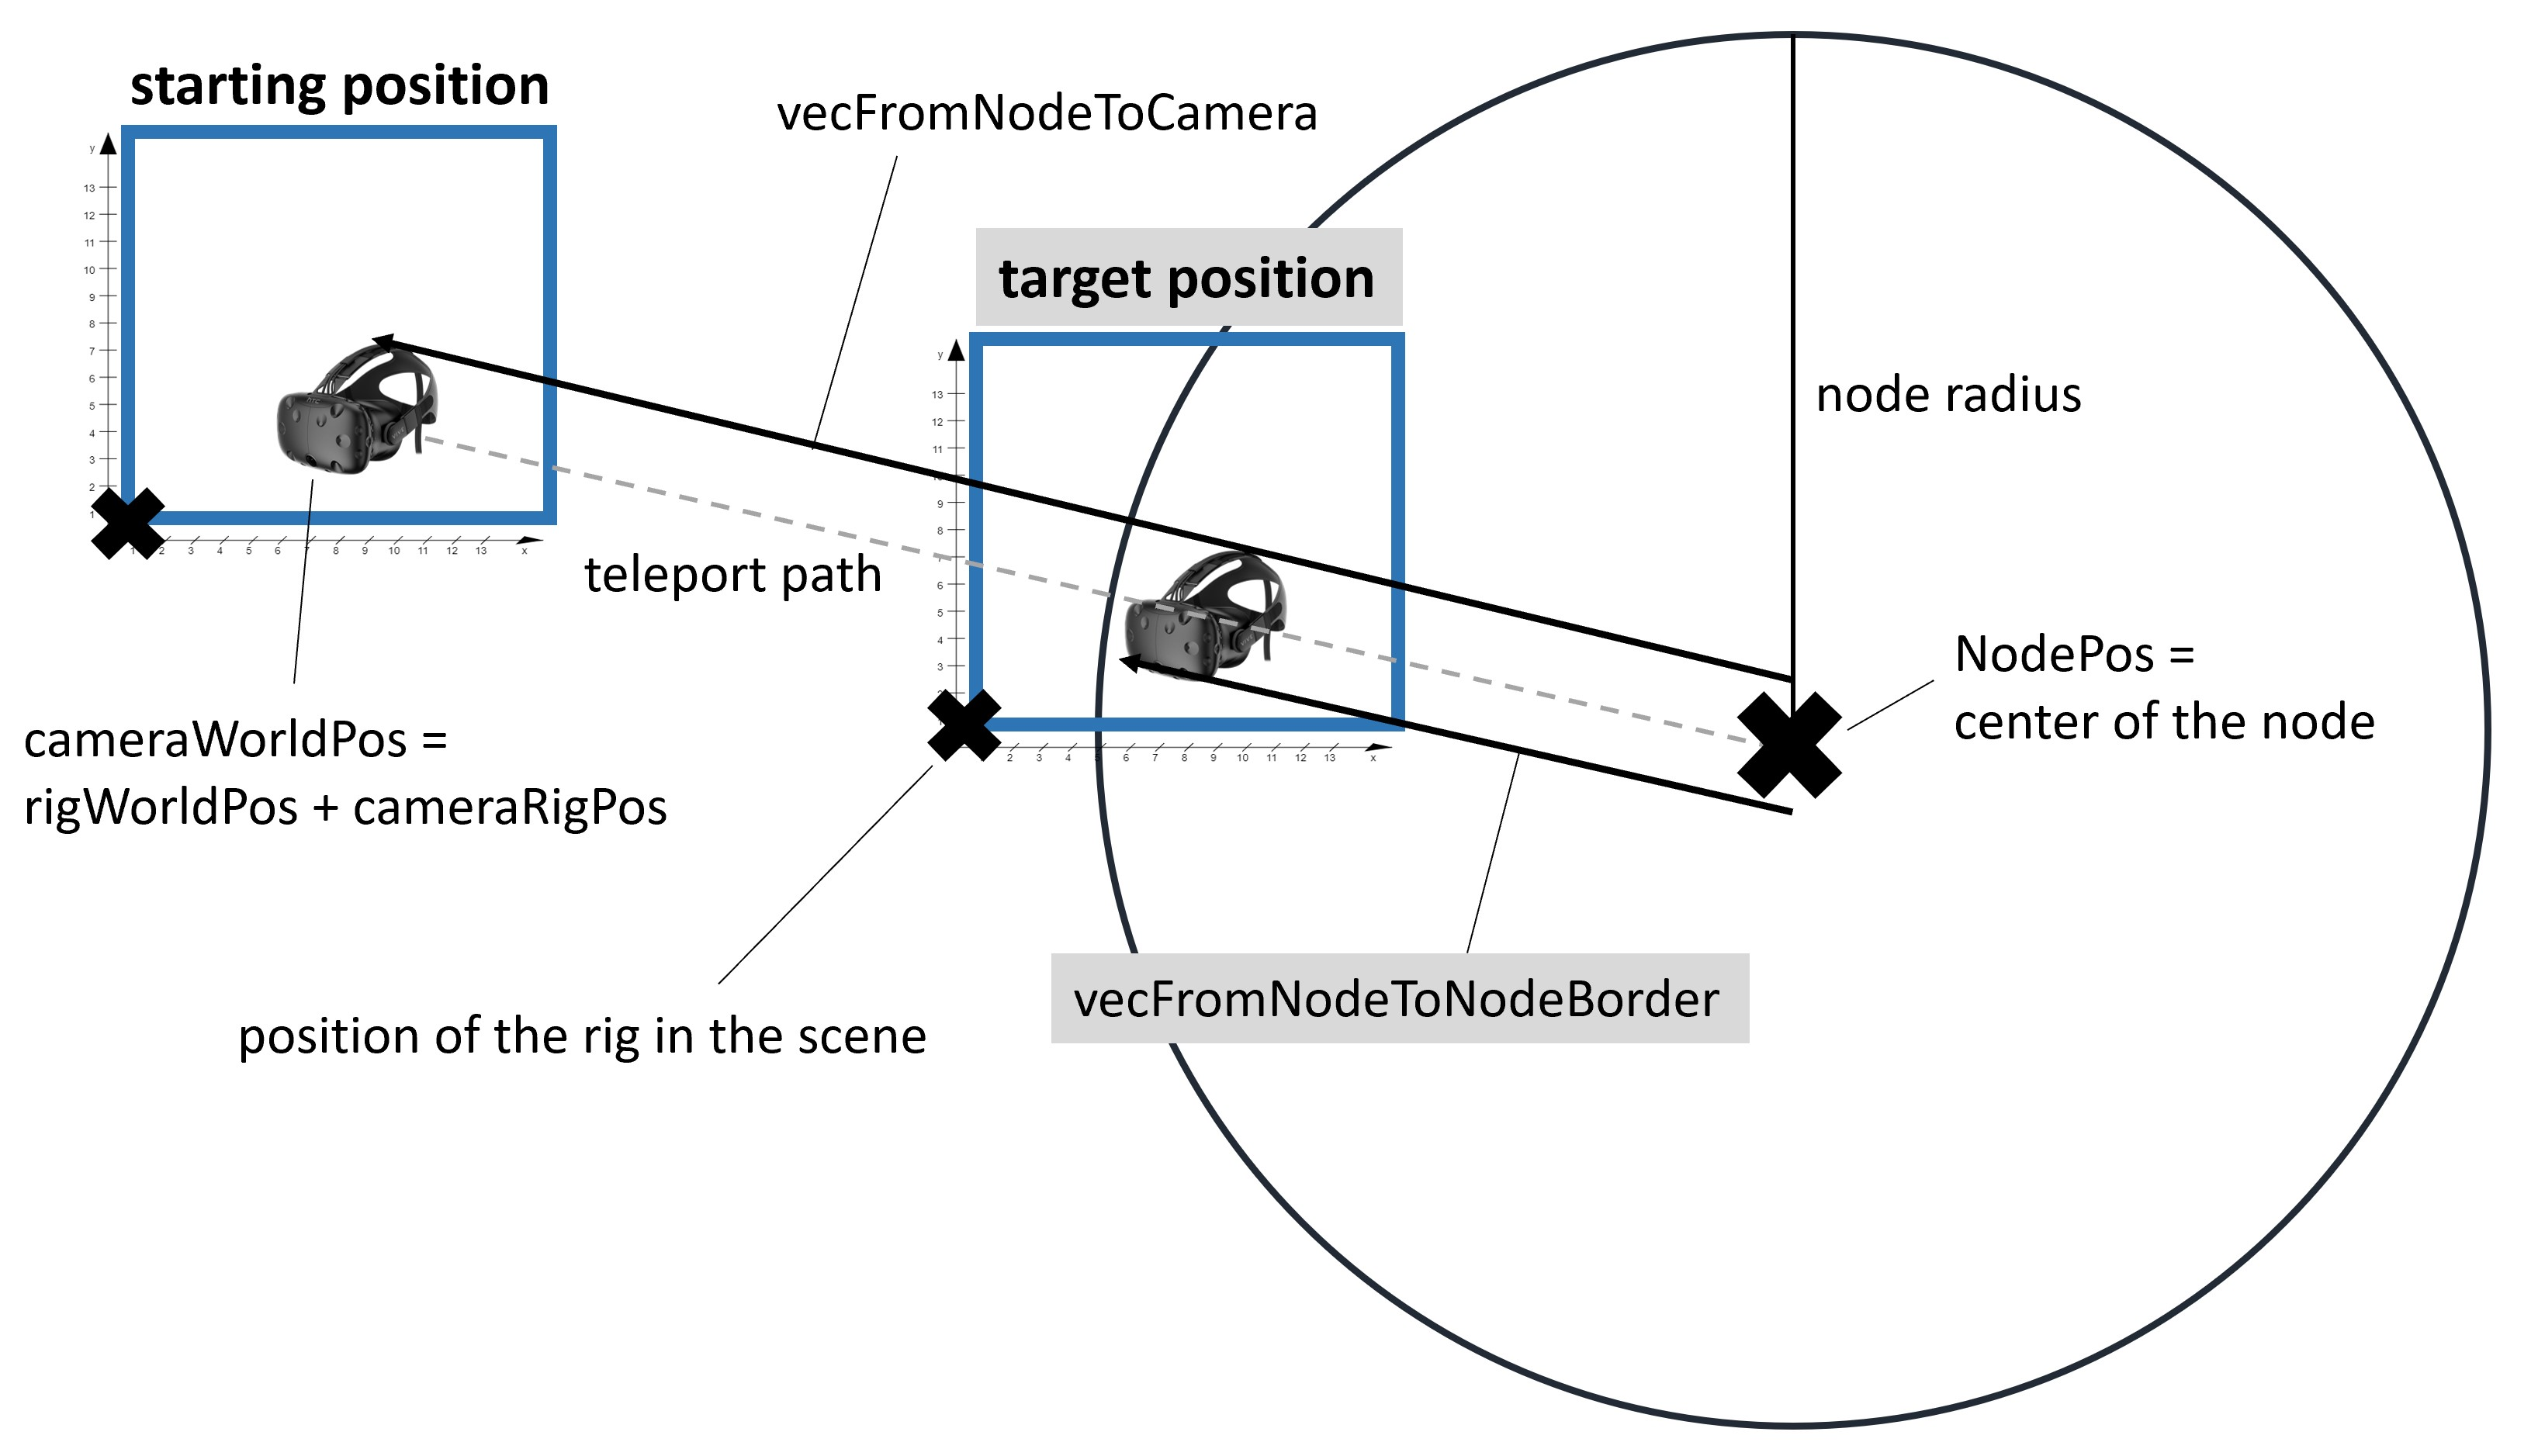
\includegraphics[width=1\textwidth]{graphics/flyToNodePositionCalc.jpg}
    \caption[2D representation of the calculation for the target position for the animated teleport.]{2D representation of the calculation for the target position for the animated teleport. A virtual teleport path is formed between the center of the node and the position of the headset. This virtual path is extended until it reaches the border of the node.} 
    \label{fig:vrFlyToNode} 
\end{figure}

In a first step, we get all information needed including the camera position in world space, the position of the node center, the node radius and the current adaptable scale of the scene.
Then we calculate the position of the crossing between the node border and the direct path from the camera to the node center. We do this by calculating a vector from the node center to the camera position. After normalizing the length and applying this vector with the correct length, determined by the node radius and scene scale, to the center of the node, we get the position where the headset should end up when teleporting to the selected node.
We can only manipulate the headset position indirectly through changing the rig position. Therefore, we have to calculate the relative rig position in the third step. 
The resulting position contains the final coordinates for centering the rig so that the VR headset ends up barely inside the node.
For calculating the target position when flying to the parent node, we apply a similar technique shown in Figure \ref{fig:vrFlyToParentNode}.

\begin{figure}[h]
    \centering
    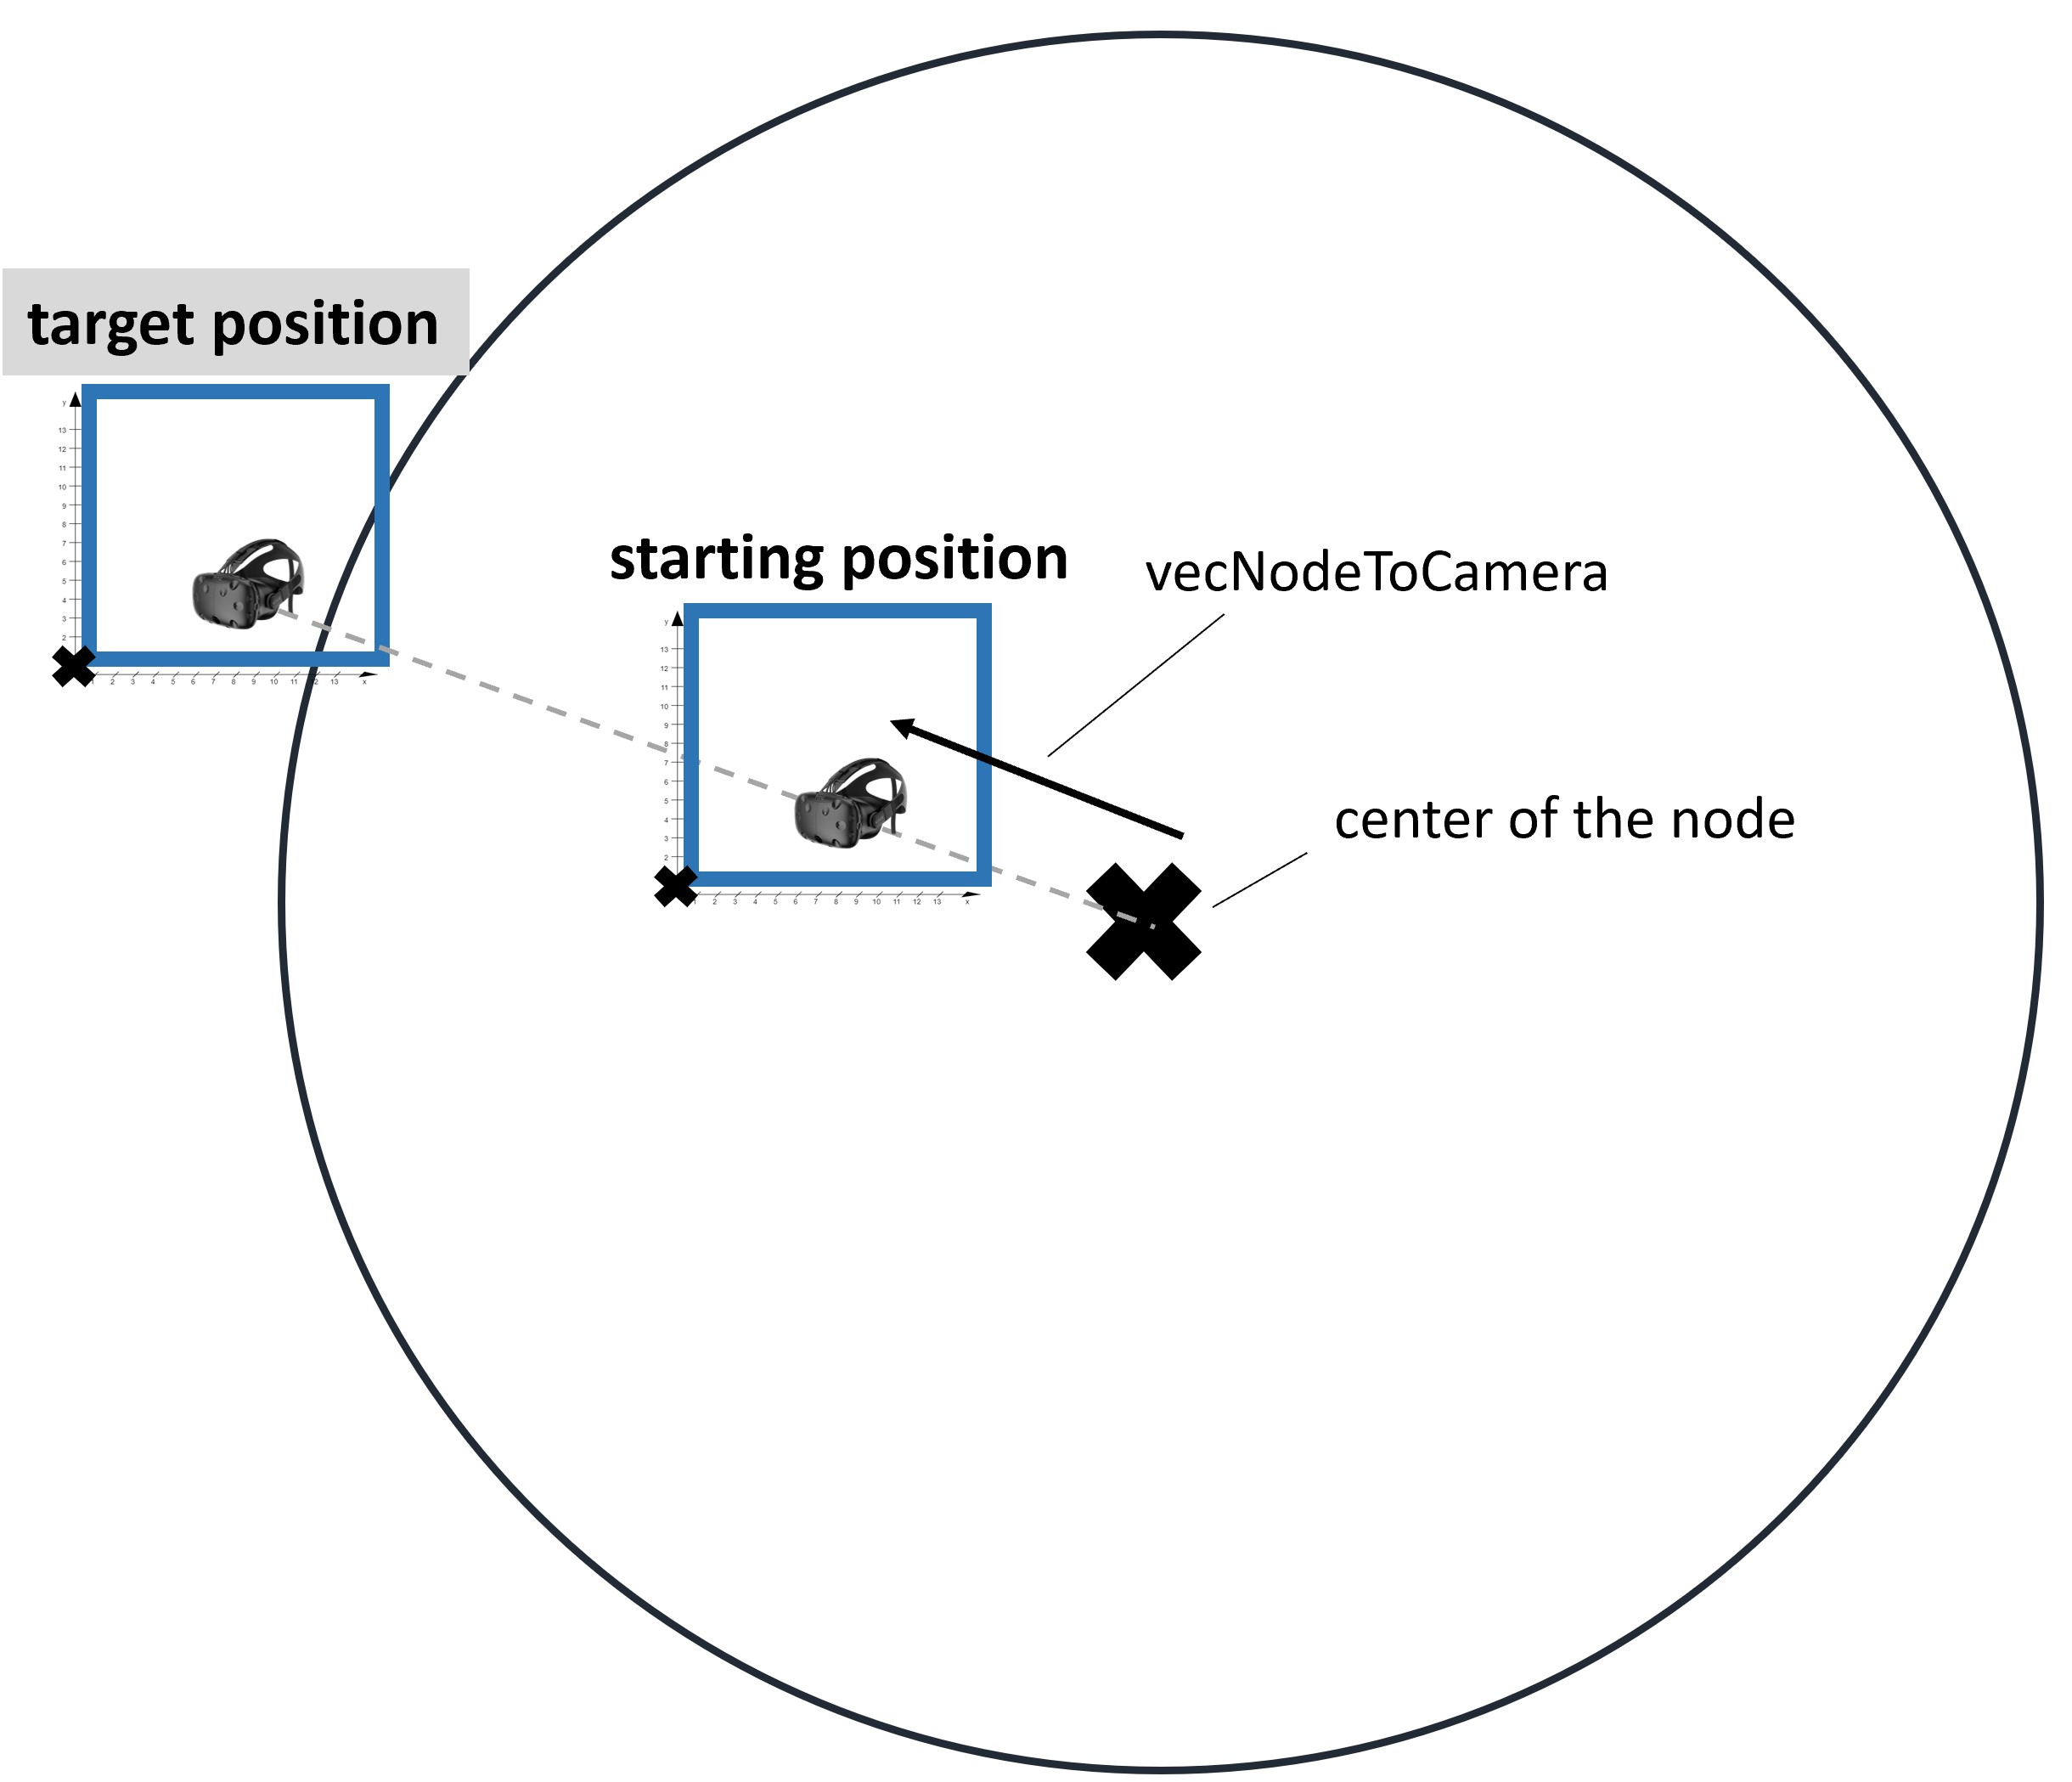
\includegraphics[width=0.75\textwidth]{graphics/flyToParentNode.jpg}
    \caption{2D representation for calculating the teleporting positing when teleporting to the parent node.} 
    \label{fig:vrFlyToParentNode} 
\end{figure}

\pagebreak

\subsection{Scaling of the Virtual Scene}
\label{sec:scaling}

In Section \ref{chap:ps-spatialReference}, we described why it is necessary to scale up the entire scene while navigating through the graph. 
The challenge while scaling is that the user's relative position in comparison the to virtual scene must not change. Otherwise, the user will get distracted while exploring.
When applying a scaling matrix, the center of the scene (0,0,0) stays in the same position. All other points are moved during the scaling process. 
Therefore, we translate the target position of the animated teleport into the center of the scene, then scale up/down and afterwards translate the scene back.
In order to achieve a smooth user-friendly scaling, instead of scaling to the desired size once, we animate the scaling process. The duration of the animation has to be the exact time as the animated teleportation. 
Otherwise, the teleportation path will get distorted and result in a curve instead of a straight line.
For manual scaling, instead of using the target position, we use the world position of the headset for translating before and after scaling. Both calculations can be seen in Listing \ref{lst:scaling}.
\pagebreak

\begin{lstlisting}[language=JavaScript,label={lst:scaling},caption=Simplified algorithm for calculating the scaling matrix]
const resultScalingMatrix = new THREE.Matrix4();
if(scalingPos === undefined){//manual scaling
    resultScalingMatrix
        .multiply(translateMatrixRig)//translate rig to center
        .multiply(translateMatrixCam)//translate cam to center
        .multiply(scaleMatrix)//scale from the center
        .multiply(reverseTranslationMatrixCam)//reverse cam translation
        .multiply(reverseTranslationMatrixRig);//reverse rig translation
}else{//automated scaling while animated teleportation
    resultScalingMatrix
        .multiply(translationMatrix)//translate target position (of teleport) to center
        .multiply(scaleMatrix)//scale from the center
        .multiply(reverseTranslationMatrix);//reverse translation
}
return resultScalingMatrix;
\end{lstlisting}

\pagebreak

\subsection{Filtering Visible Links}
\label{sec:linkFiltering}

In our visualization, links can be filtered by two ways: either by directly selecting a node, which is accomplishment with the virtual laser pointer and ray casting, or by an automated process, which selects the inner-most node related to the user's position if no node is directly selected.
In order to determine the inner-most node, we first have to check for every node if the user is inside it or not (see Listing \ref{lst:checkInsideNode}). We store all entered nodes in a temporary node cache in order to calculate the inner-most node (see Listing \ref{lst:determineInnestNode}).
Then we use that determined node to update the visibility of all links with the rules described in Section \ref{chap:ps-filterLinks}.

\begin{lstlisting}[language=JavaScript,label={lst:checkInsideNode},caption=Simplified algorithm to determine whenether the user is inside a node or not.]
//called for every frame
for (var i = 0; i < graphData.nodes.length; i++) {
    ...
    var dist = nodePos.distanceTo(getCurrentCameraRigWorldPos().add(getRelativeCameraToRigPos()));
    var threshold = multilayerNodeDiameter(node) * sceneScale;
    if (dist <= threshold) {
        detailLayout.onEnterNode(node);
    }else{
        detailLayout.onLeaveNode(node);
    }
}
\end{lstlisting}


\begin{lstlisting}[language=JavaScript,label={lst:determineInnestNode},caption=Simplified algorithm to determine the inner most node.] 
getCurrentInnestNode(){
    let innestNode = {id:"-",layer:-1};
    for (let enteredNodesKey in this.enteredNodes) {
        if(innestNode.layer < parseInt(this.enteredNodes[enteredNodesKey])){
            innestNode.id = enteredNodesKey;
        }
    }
    return this.nodeCache[innestNode.id];
}
\end{lstlisting}
